\documentclass[11pt]{article}

%%METADATA
\title{GA2001 Econometrics (Part 2) \\Solution to Problem Set 3}
\author{
Junbiao Chen\thanks{E-mail: jc14076@nyu.edu.}
}
\date{\today}


%%PACKAGES
\usepackage{mdframed} % For boxed environments
\usepackage{graphicx}
\usepackage{grffile}
\usepackage{tabularx}
\usepackage{setspace}
\usepackage{amsmath,amsthm,amssymb}
\usepackage[hyphens]{url}
\usepackage{natbib}
\usepackage[font=normalsize,labelfont=bf]{caption}
\usepackage[margin=1in]{geometry}
\usepackage{hyperref}
\hypersetup{colorlinks=true,urlcolor=blue,citecolor=blue}
\usepackage{stmaryrd}  %Package with \boxast command
\usepackage{enumerate}% http://ctan.org/pkg/enumerate %Supports lowercase Roman-letter enumeration
\usepackage{verbatim} %Package with \begin{comment} environment
%\usepackage{enumitem}
\usepackage{physics}
\usepackage{tikz}
\usepackage{pgfplots}
\pgfplotsset{compat=1.17}
\usepackage{listings}
\usepackage{xcolor}
\usepackage{upquote}
\usepackage{booktabs} %Package with \toprule and \bottomrule
\usepackage{etoc}     %Package with \localtableofcontents
\usepackage{placeins}    %Package that prevent repositioning the tables
\usepackage{multicol}
\usepackage{bm}
\usepackage{subfig}
\usepackage{csquotes}

\definecolor{dkgreen}{rgb}{0,0.6,0}
\definecolor{gray}{rgb}{0.5,0.5,0.5}
\definecolor{mauve}{rgb}{0.58,0,0.82}

\lstset{language=bash,
  frame=tb,
  aboveskip=3mm,
  belowskip=3mm,
  showstringspaces=false,
  columns=flexible,
  basicstyle={\small\ttfamily},
  numbers=none,
  numberstyle=\tiny\color{gray},
  keywordstyle=\color{blue},
  commentstyle=\color{dkgreen},
  stringstyle=\color{mauve},
  breaklines=true,
  breakatwhitespace=false,
  tabsize=3
}

\lstset{language=C,
  aboveskip=3mm,
  belowskip=3mm,
  showstringspaces=false,
  columns=flexible,
  basicstyle={\small\ttfamily},
  numbers=none,
  numberstyle=\tiny\color{gray},
  keywordstyle=\color{blue},
  commentstyle=\color{dkgreen},
  stringstyle=\color{mauve},
  breaklines=true,
  breakatwhitespace=false,
  tabsize=4
}

% Define Julia style for lstlisting
\lstdefinelanguage{Julia}{
    morekeywords={
        for, end, in, if, else, elseif, while, break, continue, return, function,
        struct, mutable, begin, do, using, import, export, const, let, local, global,
        try, catch, finally, true, false, nothing, quote, macro, module, baremodule,
        where, abstract, typealias, type, bitstype
    },
    sensitive=true,
    morecomment=[l]{\#},
    morestring=[b]",
    morestring=[b]',
}

\lstset{
    language=Julia,
    basicstyle=\ttfamily\footnotesize,
    keywordstyle=\color{blue}\bfseries,
    commentstyle=\color{gray}\itshape,
    stringstyle=\color{red},
    numbers=left,
    numberstyle=\tiny\color{gray},
    stepnumber=1,
    numbersep=5pt,
    showspaces=false,
    showstringspaces=false,
    breaklines=true,
    breakatwhitespace=true,
    frame=single,
    captionpos=b
}


\definecolor{lightblue}{rgb}{0.68, 0.85, 0.9} %

%CUSTOM DEFINITIONS
\theoremstyle{definition}
\newtheorem{definition}{Definition}[section]
\newtheorem*{remark}{Remark}
\setcounter{secnumdepth}{3}
\usepackage{tikz}
\usetikzlibrary{arrows.meta}
\usetikzlibrary{automata, positioning, arrows, calc}

\tikzset{
	->,  % makes the edges directed
	>=stealth, % makes the arrow heads bold
	shorten >=2pt, shorten <=2pt, % shorten the arrow
	node distance=3cm, % specifies the minimum distance between two nodes. Change if n
	every state/.style={draw=blue!55,very thick,fill=blue!20}, % sets the properties for each ’state’ n
	initial text=$ $, % sets the text that appears on the start arrow
 }

%% PROPOSITION
% Define the Proposition environment
\newmdenv[
  innerleftmargin=10pt, 
  innerrightmargin=10pt,
  innertopmargin=10pt,
  innerbottommargin=10pt,
  linecolor=black, 
  linewidth=1pt,
  backgroundcolor=white, 
  roundcorner=5pt
]{propositionbox}

\newtheoremstyle{boldtitle} % Define a new theorem style
  {10pt} % Space above
  {10pt} % Space below
  {\itshape} % Body font
  {} % Indent amount
  {\bfseries} % Theorem head font
  {.} % Punctuation after theorem head
  { } % Space after theorem head
  {} % Theorem head spec

\theoremstyle{boldtitle} % Use the custom style
\newtheorem{proposition}{Proposition} % Define the proposition environment

% Redefine the proposition environment to use the box
\newenvironment{boxedproposition}[1][]
{\begin{propositionbox}\begin{proposition}[#1]}
{\end{proposition}\end{propositionbox}}

%%FORMATTING
\usepackage[bottom]{footmisc}
\onehalfspacing
\numberwithin{equation}{section}
\numberwithin{figure}{section}
\numberwithin{table}{section}
\bibliographystyle{../bib/aeanobold-oxford}


%main text
\begin{document}
\maketitle
\section*{Problem 1. Testing Linear Restriction}
\subsection*{(a) Answer} 
The Lagragian is given by 
\[
\mathcal{L} = \frac{1}{2} (y - X\beta)' (y - X \beta) + \lambda (R\beta -r),
\]
where $\lambda \in \mathbb{R}^q$.

The FOC is 
\[
-X'(y - X \hat{\beta}_{CLS}) + R' \hat{\lambda}_{CLS} = 0 
\]
It follows that 
\begin{align}
    \label{eqn:FOC}
    -X'y + X'X\hat{\beta}_{CLS} +  R' \hat{\lambda}_{CLS} = 0
\end{align}
Pre-multiplying both sides by $R(X'X)^{-1}$ (because I want to use the linear restriction to simplify terms),
then we have:
\begin{align*}
    & -R(X'X)^{-1}X'y + R(X'X)^{-1}X'X\hat{\beta}_{CLS} + R(X'X)^{-1}R' \hat{\lambda}_{CLS} = 0 \\ 
\Rightarrow & - R \hat{\beta}_{LS} + r + R(X'X)^{-1}R' \hat{\lambda}_{CLS} = 0 \\ 
\Rightarrow & - \hat{d} + R(X'X)^{-1}R' \hat{\lambda}_{CLS} = 0
\end{align*}
Therefore, we have 
\[
\hat{\lambda}_{CLS} = \left[R(X'X)^{-1}R' \right]^{-1}\hat{d}
\]
Plugging it back to equation~(\ref{eqn:FOC}), we have 
\begin{align*}
\hat{\beta}_{CLS} & = (X'X)^{-1}X'y - (X'X)^{-1} R' \left[R(X'X)^{-1}R' \right]^{-1}\hat{d} \\ 
    & = \hat{\beta}_{LS} - (X'X)^{-1} R' \left[R(X'X)^{-1}R' \right]^{-1}\hat{d}
\end{align*}
Now expressing $\hat{e}_R$ using 
$\hat{e}_R = y - X\hat{\beta}_{CLS} = \hat{e}_R +  X(\hat{\beta}_{LS} - \hat{\beta}_{CLS}),$
then we have 
\[
\hat{e}_R = \hat{e}_u +  X(X'X)^{-1} R' \left[R(X'X)^{-1}R' \right]^{-1}\hat{d}
\]
\(\blacksquare\)

\subsection*{(b) Answer} 
Following (a), we have 
\begin{align*}
    \hat{e}_R' \hat{e}_R & = \left[\hat{e}_u +  X(X'X)^{-1} R' \left[R(X'X)^{-1}R' \right]^{-1}\hat{d} \right]'
    \left[\hat{e}_u +  X(X'X)^{-1} R' \left[R(X'X)^{-1}R' \right]^{-1}\hat{d} \right] \\ 
    & = \hat{e}_u'\hat{e}_u + \hat{d}'\left[R(X'X)^{-1}R' \right]^{-1} R(X'X)^{-1} X'  X(X'X)^{-1} R' \left[R(X'X)^{-1}R' \right]^{-1}\hat{d}  \\ 
    & = \hat{e}_u'\hat{e}_u + \hat{d}'\left[R(X'X)^{-1}R' \right]^{-1} \hat{d}  \\ 
\end{align*}

\subsection*{(c) Answer} 
Given the results in (b), we can express the Wald, the LM, and the LR statistics as follows.

\noindent \textbf{The Wald statistic:}
\begin{align*}
    W_n & = n (R \hat{\beta}_{LS} - r)' \hat{V}_r^{-1} (R \hat{\beta}_{LS} - r) \\ 
      & = n (R \hat{\beta}_{LS} - r)' \left(R \hat{V}_\beta R'\right)^{-1} (R \hat{\beta}_{LS} - r) \\ 
    & = n \hat{d}'\bigg[R \frac{n }{n - k} \hat{e}_u'\hat{e}_u (X'X)^{-1}R' \bigg]^{-1} \hat{d} \\
    & = (n - k) \left(\hat{e}_u'\hat{e}_u \right)^{-1}  \hat{d}' \bigg[R (X'X)^{-1}R' \bigg]^{-1} \hat{d}
\end{align*}
Using the result in (b), we have 
\[
W_n = (n - k)  \frac{\hat{e}_R' \hat{e}_R - \hat{e}_u'\hat{e}_u}{\hat{e}_u'\hat{e}_u},
\]
which is also known as the \textit{F-statistic}.


\noindent \textbf{The LM statistic:}
Compared to the Wald statistic, 
the LM statistic is replacing the un-restricted residuals with the restricted one, we have 
\begin{align*}
    LM_n & = (n - k) \left(\hat{e}_R'\hat{e}_R \right)^{-1}  \hat{d}' \bigg[R (X'X)^{-1}R' \bigg]^{-1} \hat{d} \\ 
    & =  (n - k)  \frac{\hat{e}_R' \hat{e}_R - \hat{e}_u'\hat{e}_u}{\hat{e}_R'\hat{e}_R}
\end{align*}


\noindent \textbf{The LR statistic:}
Using the result derived in class, we have 
\begin{align*}
LR_n & = n \log \left(\frac{\hat{\sigma}_R^2}{\hat{\sigma}_u^2} \right) \\ 
  & =  n \log \left(\frac{\hat{e}_R' \hat{e}_R }{\hat{e}_u'\hat{e}_u} \right)
\end{align*}


\subsection*{(d) Answer} 
Since $\frac{\hat{e}_R' \hat{e}_R - \hat{e}_u'\hat{e}_u}{\hat{e}_R'\hat{e}_R} < 1$, 
we can depict $W_n, LM_n, LR_n$ in the following figure and conclude that 
\[
W_n > LR_n > LM_n \quad \text{with } (n \gg k)
\] 


\begin{center}
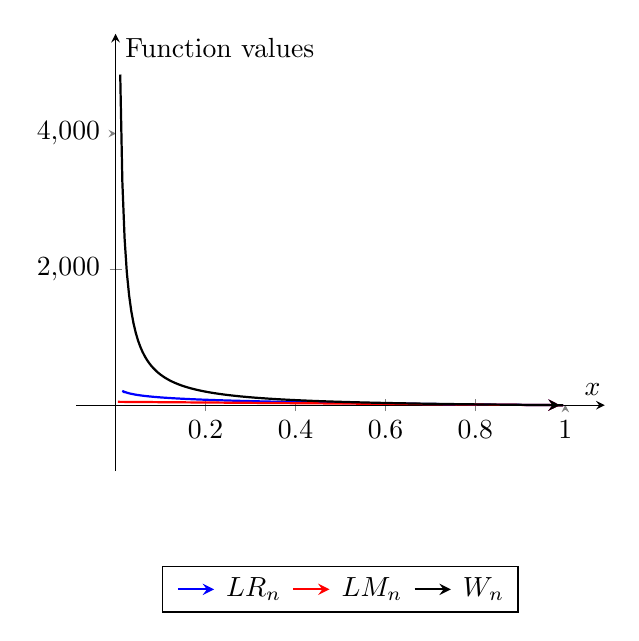
\begin{tikzpicture}
    \begin{axis}[
        xlabel={$x$},
        ylabel={Function values},
        xmin=0, xmax=1,
        ymin=-500, ymax=5000, % Rescaled y-axis
        legend style={at={(0.5,-0.2)}, anchor=north, legend columns=-1},
        axis lines=middle,
        enlargelimits=true,
        no markers
    ]
        % Plot LR_n = -n log(x), n=100
        \addplot[blue, thick, domain=0.01:1, samples=200] {-50*ln(x)};
        \addlegendentry{$LR_n$}

        % Plot LM_n = n(1-x), n=100
        \addplot[red, thick, domain=0:1, samples=200] {50*(1-x)};
        \addlegendentry{$LM_n$}

        % Plot W_n = n(1/x - 1), n=100
        \addplot[black, thick, domain=0.01:1, samples=200] {50*(1/x - 1)};
        \addlegendentry{$W_n $}
    \end{axis}
\end{tikzpicture}
\end{center}



\section{Problem 2. Bootstrap}
\subsection{(a) - (c)}
\begin{lstlisting}[language=Julia, caption=Residual Bootstrap Code]
# Residual bootstrap (part a, b, c)
for n in [10, 50, 200]
    Random.seed!(n) 
    x = rand(Uniform(0,2), n)

    Random.seed!(n+1)
    e = rand(Uniform(-1,1), n)
    y = beta_zero .+ beta_one .* x .+ e

    S = 202  # Number of bootstrap replications
    x_cat = hcat(ones(n), x)
    beta_hat, var_beta_hat, residuals = ls_estimator(y, x_cat)

    # Bootstrap distributions
    beta_one_hat_bs = zeros(S)
    t_stat_bs = zeros(S)

    for s in 1:S
        Random.seed!(s)
        e_sim = rand(residuals, n)
        y_sim = x_cat * beta_hat .+ e_sim
        beta_hat_bs, var_beta_hat_bs, _ = ls_estimator(y_sim, x_cat)
        beta_one_hat_bs[s] = beta_hat_bs[2]
        beta_one_std_bs = sqrt(var_beta_hat_bs[2, 2])
        t_stat_bs[s] = t_ratio(beta_hat_bs[2], beta_one, beta_one_std_bs)
    end

    t_stat_bs = sort(t_stat_bs)[2:end-1]
    beta_one_hat_bs = sort(beta_one_hat_bs)[2:end-1]

    # Compute 95th percentiles of bootstrap distributions
    beta_one_95_bs = quantile(beta_one_hat_bs, 0.95)
    t_stat_95_bs = quantile(t_stat_bs, 0.95)

    # Visualization
    p1 = histogram(beta_one_hat_bs, xlims=(0, 2), label="Bootstrap beta_one_hat", color=:blue, alpha=0.6)
    vline!(p1, [beta_one_95_bs], label="95th Percentile", color=:red, linestyle=:dash, linewidth=3)
    annotate!(p1, [(beta_one_95_bs, 3, text(string(round(beta_one_95_bs, digits=3)), :black, 12, :bold))])

    p2 = histogram(t_stat_bs, xlims=(0, 4), label="Bootstrap t-stat", color=:green, alpha=0.6)
    vline!(p2, [t_stat_95_bs], label="95th Percentile", color=:red, linestyle=:dash, linewidth=3)
    annotate!(p2, [(t_stat_95_bs, 3, text(string(round(t_stat_95_bs, digits=3)), :black, 12, :bold))])

    plot(p1, p2,
        layout=(1, 2),
        xlabel="Value",
        ylabel="Frequency",
        size=(800, 300)
    )
end
\end{lstlisting}

\subsection{(d). Answer}
\begin{figure}[htbp]
  \centering
  \includegraphics[width=0.9\textwidth]{bootstrap/images/bootstrap_n10.png}
  \caption{Residual Bootstrap (n = 10)}
  \begin{minipage}{0.95\textwidth}{\footnotesize \textsc{Notes}:
   The figures above display the distribution of the simulated distribution based on residual bootstrap.
  \par}\end{minipage}
\end{figure}

\begin{figure}[htbp]
  \centering
  \includegraphics[width=0.9\textwidth]{bootstrap/images/bootstrap_n50.png}
  \caption{Residual Bootstrap (n = 50)}
  \begin{minipage}{0.95\textwidth}{\footnotesize \textsc{Notes}:
   The figures above display the distribution of the simulated distribution based on residual bootstrap.
  \par}\end{minipage}
\end{figure}

\begin{figure}[htbp]
  \centering
  \includegraphics[width=0.9\textwidth]{bootstrap/images/bootstrap_n200.png} 
  \caption{Residual Bootstrap (n = 200)}
  \begin{minipage}{0.95\textwidth}{\footnotesize \textsc{Notes}:
   The figures above display the distribution of the simulated distribution based on residual bootstrap.
  \par}\end{minipage}
\end{figure}

\begin{figure}[htbp]
  \centering
  \includegraphics[width=0.9\textwidth]{bootstrap/images/condition_dist_based_n10.png}
  \caption{Simulations based on conditional distribution (n = 10)}
  \begin{minipage}{0.95\textwidth}{\footnotesize \textsc{Notes}:
   The figures above display the distribution of the simulated distribution based on residual bootstrap.
  \par}\end{minipage}
\end{figure}

\begin{figure}[htbp]
  \centering
  \includegraphics[width=0.9\textwidth]{bootstrap/images/condition_dist_based_n50.png}  
  \caption{Simulations based on conditional distribution (n = 50)}
  \begin{minipage}{0.95\textwidth}{\footnotesize \textsc{Notes}:
   The figures above display the distribution of the simulated distribution based on residual bootstrap.
  \par}\end{minipage}
\end{figure}

\begin{figure}[htbp]
  \centering
  \includegraphics[width=0.9\textwidth]{bootstrap/images/condition_dist_based_n50.png}  
  \caption{Simulations based on conditional distribution (n = 200)}
  \begin{minipage}{0.95\textwidth}{\footnotesize \textsc{Notes}:
   The figures above display the distribution of the simulated distribution based on residual bootstrap.
  \par}\end{minipage}
\end{figure}

\clearpage
\section{Problem 3. 2SLS and IV}
\subsection{(a). Answer}
Recall that the rank condition is given by 
\[
\text{rank}\left(\mathbb{E}(z_i x_i') \right) = m
\]
Then, in the context of problem 3, we have 
\[
\text{rank}\left(
    \begin{bmatrix}
        1 & \mathbb{E}(x_{i2}) \\ 
        \mathbb{E}(z_{i2}) & \mathbb{E}(z_{i2} x_{i2})
    \end{bmatrix}
    \right) = 2
\]
It follows that 
\[
\text{rank}\left(
    \begin{bmatrix}
        1 & \mathbb{E}(x_{i2}) \\ 
        \mathbb{E}(z_{i2}) & \text{Cov}(z_{i2}, x_{i2}) + \mathbb{E}(z_{i2}) \mathbb{E}(x_{i2})
    \end{bmatrix}
    \right) = 2
\]
which holds iff $\text{Cov}(z_{i2}, x_{i2}) \neq 0$. \(\blacksquare\)


\subsection{(b). Answer}
Since $m = k = 2$, the inverse of $Z'X$ exists. 
Therefore, we have 
\begin{align*}
\hat{\beta}_{2SLS} & = (X'Z(Z'Z)^{-1}Z'X)^{-1} X'Z(Z'Z)^{-1}Z'y \\ 
& = (Z'X)^{-1} Z'y \\ 
& = \begin{bmatrix}
        \frac{\sum_i^n y_i}{n} \\ 
        \frac{\sum_i^n z_{i,2} y_i}{\sum_i^n z_{i,2} x_{i,2}}
    \end{bmatrix}
\end{align*}
Hence, we have 
\[
\hat{\beta}_{2, 2SLS} = \frac{\text{Cov}(z_{i,2}, y)}{\text{Cov}(z_{i, 2}, x_{i, 2})}
\]

\subsection{(c). Answer}
In the general case that includes both ``just-identification'' and ``over-identification'',
we have 
\[
A'Z'(y - X' \hat{\beta}_{IV}) = 0
\]
It follows that 
\[
\hat{\beta}_{IV} = \left(A'Z'X \right)^{-1} \left(A'Z'y \right)
\]

\subsection{(d). Answer}
Since the structural model is given by $x'_i = z'_i \Pi + v'_i$, we have 
\begin{align*}
    & P_Z X = Z \hat{\Pi} \\ 
    \Rightarrow & X'P_Z = X' P_Z = \hat{\Pi}' Z' 
\end{align*}
Therefore, the 2SLS estimator is given by 
\begin{align*}
\hat{\beta}_{2SLS} & = (X'P_Z X)^{-1} X'P_Z y     \\ 
    & =  (\hat{\Pi}' Z' X)^{-1} \hat{\Pi}' Z' y
\end{align*}
which is equivalent to the IV estimator when $A = \hat{\Pi}$:
\[
\hat{\beta}_{IV} = \left(\hat{\Pi}' Z'X \right)^{-1} \left(\hat{\Pi}' Z'y \right)
\]


\section{Problem 4. Nonlinear Transformations}
\subsection{(a). Answer}
Yes. We can prove the consistency of the 2SLS estimator using LLN under standard regularity assumptions:
\begin{align*}
    \hat{\beta}_{2SLS} - \beta & = (X'Z(Z'Z)^{-1}Z'X)^{-1} X'Z(Z'Z)^{-1}Z'e \\ 
    & = \left(\frac{X'Z}{n}\left(\frac{Z'Z}{n}\right)^{-1}\frac{Z'X}{n}\right)^{-1} \frac{X'Z}{n}\left(\frac{Z'Z}{n}\right)^{-1}\frac{Z'e}{n} \\
    & \rightarrow_p \left(\mathbb{E}[Z_i X_i']' \mathbb{E}[Z_i Z_i']^{-1} \mathbb{E}[Z_i X_i'] \right)^{-1} 
    \mathbb{E}[Z_i X_i']' \mathbb{E}[Z_i Z_i']^{-1} \mathbb{E}[Z_i e_i] = 0
\end{align*}


\subsection{(b). Answer}
No! This procedure is known as the ``forbidden regression''.
Let $\hat{\pi}$ be the first stage coefficient.
Denote the following by $\hat{X}$ 
\[
\hat{X} = \begin{bmatrix}
    1 & \hat{\pi} z_1 & \hat{\pi}^2 z_1^2 \\ 
    1 & \hat{\pi} z_2 & \hat{\pi}^2 z_2^2 \\ 
    \vdots \\
    1 & \hat{\pi} z_n & \hat{\pi}^2 z_n^2 \\ 
\end{bmatrix}
\]
Then, the coefficient of the second stage is given by 
\[
\hat{\beta} = (\hat{X}'\hat{X})^{-1} (\hat{X}' y)
\]
It follows that 
\begin{align*}
\hat{\beta} - \beta & = (\hat{X}'\hat{X})^{-1} (\hat{X}' (X \beta + e)) \\ 
& = \begin{bmatrix}
    n & \hat{\pi} \sum_i z_i & \hat{\pi}^2 \sum_i z_i^2 \\ 
    \hat{\pi} \sum_i z_i & \hat{\pi}^2 \sum_i z_i^2 & \hat{\pi}^3 \sum_i z_i^3 \\ 
    \hat{\pi}^2 \sum_i z_i^2 & \hat{\pi}^3 \sum_i z_i^3 & \hat{\pi}^4 \sum_i z_i^4 \\ 
\end{bmatrix}^{-1}
\begin{bmatrix}
    n & \hat{\pi} \sum_i x_i & \hat{\pi}^2 \sum_i x_i^2 \\ 
    \hat{\pi} \sum_i z_i & \hat{\pi}^2 \sum_i z_i x_i & \hat{\pi} \sum_i z_i x_i^2 \\ 
    \hat{\pi}^2 \sum_i z_i^2 & \hat{\pi}^2 \sum_i z_i^2 x_i & \hat{\pi}^2 \sum_i z_i^2 x_i^2 \\ 
\end{bmatrix}
\begin{bmatrix}
    \beta_0 \\ 
    \beta_1 \\ 
    \beta_2  \\ 
\end{bmatrix}
\\ 
\\
&\quad + \begin{bmatrix}
    n & \hat{\pi} \sum_i z_i & \hat{\pi}^2 \sum_i z_i^2 \\ 
    \hat{\pi} \sum_i z_i & \hat{\pi}^2 \sum_i z_i^2 & \hat{\pi}^3 \sum_i z_i^3 \\ 
    \hat{\pi}^2 \sum_i z_i^2 & \hat{\pi}^3 \sum_i z_i^3 & \hat{\pi}^4 \sum_i z_i^4 \\ 
\end{bmatrix}^{-1}
\begin{bmatrix}
    \sum_i^n e_i \\ 
    \hat{\pi} \sum_i^n z_i e_i \\ 
    \hat{\pi} \sum_i^n z_i^2 e_i^2  \\ 
\end{bmatrix}
\end{align*}
By LLN, $\sum_i^n z_i^2 e_i^2 \rightarrow \mathbb{E}[z_i^2 e_i]$;
however, the linear model does NOT assume non-linear independence between $Z_i$ and $e_i$,
concretely, $\mathbb{E}[z_i^2 e_i] \neq 0$, 
the estimator $\hat{\beta}$ above is not consistent!


\subsection{(c). Answer}
There are two approaches to derive consistent estimator:
\begin{enumerate}
    \item Assume/argue that $\mathbb{E}[z_i^2 e_i] = 0$, and apply the estimator above. 
    \item Find a different instrument $\tilde{Z}_i \neq Z_i$ for $x_i^2$, and run the regular  2SLS.
\end{enumerate}


%% =========== %% ========= %%
\bibliography{../bib/notes.bib}

\end{document}